\documentclass[a4paper,11pt]{article}
\usepackage[utf8]{inputenc}
\usepackage{amssymb}
\usepackage{amsmath} 
\usepackage{enumerate}
\usepackage{tikz}

\DeclareMathOperator*{\argmax}{arg\!\max}
\DeclareMathOperator*{\argmin}{arg\!\min}
\DeclareMathOperator*{\var}{var}
\newcounter{exercise}
\setcounter{exercise}{0}
\newcounter{subexercise}
\newcommand*{\exercise}[1][]{\subsection*{Exercise \ifx/#1/\stepcounter{exercise}\arabic{exercise}\else#1\fi}\setcounter{subexercise}{0}}
\newcommand*{\subexercise}[1][]{
\par{\noindent\textbf{\ifx/#1/\protect\stepcounter{subexercise}\alph{subexercise}\else#1\fi.\quad}}}

\title{Chapter 10}
\author{stevenjin8}
\date{November 7, 2020}

\begin{document}
\maketitle

\section*{Exercises}

\exercise
Marginalizing out $X$ gives
\begin{align*}
    p(A:F) &= \sum\limits_{x'} p( A:F | X=x' ) \\
    &= p( A ) p( B ) p( C ) p( E ) \sum\limits_{x'} p( E, F | C, D, X=x' ) p( X=x'| A:D ) \\
    &= p( A ) p( B ) p( C ) p( D ) p( E, F | A:D ) \\
    &= p( A ) p( B ) p( C ) p( D ) p( F | A:E )p( E | A:D ). \\
\end{align*}
It follows that the graph $G'$ is
\begin{center}
    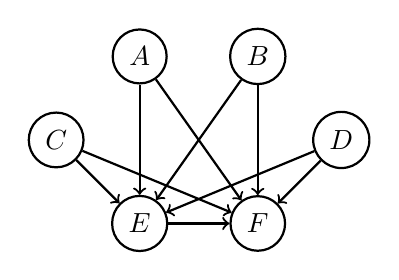
\begin{tikzpicture}[ node distance={15mm}, thick, main/.style = {draw, circle} ]
        \node[main] (1) {$A$}; 
        \node[main] (2) [right of=1] {$B$};
        \node[main] (3) [below left of=1] {$C$}; 
        \node[main] (4) [below right of=2] {$D$};
        \node[main] (5) [below right of=3] {$E$}; 
        \node[main] (6) [below left of=4] {$F$};

        \draw[->] (1) -- (5); 
        \draw[->] (1) -- (6); 
        \draw[->] (2) -- (5); 
        \draw[->] (2) -- (6); 
        \draw[->] (3) -- (5); 
        \draw[->] (3) -- (6); 
        \draw[->] (4) -- (5); 
        \draw[->] (4) -- (6); 
        \draw[->] (5) -- (6); 
    \end{tikzpicture}
\end{center}
Note that we can reverse $E \rightarrow F$.

We know that this is a minimal I-map because removing any edges creates conditional
independence assumptions not made by $G$:
\begin{center}
    \begin{tabular}{c|l|c} 
        Edge removed in $G'$ & New CI in $G'$ & Counterexample in $G$\\
         \hline
         $A\rightarrow E$ & $A \perp_{G'} E | B, C, D$ & $ A\rightarrow X \rightarrow E$ \\
         $A\rightarrow F$ & $A \perp_{G'} F | B, C, D, E$ & $A \rightarrow  X\rightarrow F$ \\
         $B\rightarrow E$ & $B \perp_{G'} E | A, C, D$ & $ B \rightarrow X \rightarrow E$ \\
         $B\rightarrow F$ & $B \perp_{G'} F | A, C, D, E$ & $ B\rightarrow X \rightarrow F$ \\
         $C\rightarrow E$ & $C \perp_{G'} E | A, B, D$ & $C \rightarrow X \rightarrow E$ \\
         $C\rightarrow F$ & $C \perp_{G'} F | A, B, D, E$ & $C \rightarrow  X\rightarrow F$ \\
         $D\rightarrow E$ & $D \perp_{G'} E | A, B, C$ & $D \rightarrow X \rightarrow E$ \\
         $D\rightarrow F$ & $D \perp_{G'} F | A, B, C, E$ & $D \rightarrow  X\rightarrow F$ \\
         $E\rightarrow F$ & $E \perp_{G'} F | A, B, C,D$ & $E \leftarrow X\rightarrow F$ \\
    \end{tabular}
\end{center}

The first row of the above table can be read as: removing the $A\rightarrow E$ edge in
$G'$ creates the conditional independence $A \perp_{G'} E | B, C, D$; however, this CI
is not held in $G$ because of the $A \rightarrow X \rightarrow E$ path.

Note that $A \perp_{G'} E | B, C, D$ rather than $A \perp_{G'} E | B, C, D, F$ because of
Berkson's paradox (this also applies for all above CIs conditioned on three nodes).

This exercise highlights the power of hidden nodes: $G'$ has 50\% more edges
than $G$, despite having fewer nodes.

\setcounter{exercise}{2}
\exercise
Let $Y_i = \text{ch}( X_i )$, $B_i = \text{pa}( X_i )$, $Z_i = \text{copa}( X_i )$,
and $U_i = X_{-i} \setminus ( Z_i \cup Z_i \cup B_i )$.
\begin{align*}
    p( X_i | X_{-i} ) &= \frac{ p( X_i, X_{-i} )}{ p( X_{-i} )} \\
    &\propto p( X_i, X_{-i} ) \\
    &= p( X_i, B_i, Y_i, Z_i, U_i ) \\
    &= p( Y_i | X_i, Z_i ) p( X_i|B_i ) p( B_i, Z_i, U_i ) \\
    &\propto p( Y_i | X_i, Z_i ) p( X_i | B_i ) \\
    &= p( X_i | B_i ) \prod\limits_{ y\in Y_i } p( y | pa(y) ).
\end{align*}
\end{document}
